\documentclass[11pt,a4paper]{article}
\usepackage[utf8]{inputenc}
\usepackage{float,graphicx,amsfonts,amsmath,amssymb,authblk,graphicx,longtable,booktabs,fullpage}
\graphicspath{ {../img/} }
\usepackage[colorlinks = true,
            linkcolor = black,
            urlcolor  = blue,
            citecolor = blue,
            anchorcolor = blue]{hyperref}

\title{Dispositivo di Fletcher}

\author[1]{Dennis Angemi}%
\author[1]{Federica Ingrassia}%
\author[1]{Giuseppe Di Silvestre}%
\author[1]{Giulia De Luca}%
\affil[1]{Dipartimento di Fisica e Astronomia ``Ettore Majorana'' - Università degli Studi di Catania}%

\date{14 Marzo 2022}

\begin{document}

\maketitle

\begin{abstract}
   
Si è verificata la dipendenza lineare tra forza e accelerazione dalla misura dei tempi impiegati da un carrello a percorrere un piano in assenza di attrito. Successivamente si è calcolato il valore della massa del carrello e i valori ottenuti risultano essere in buon accordo con il valore aspettato.
   
\end{abstract}

\section{Introduzione e cenni teorici}
La Macchina di Fletcher è un dispositivo che studia e analizza il secondo principio della dinamica, cioè la proporzionalità diretta tra la forza applicata ad un punto materiale e l'accelerazione che si ottiene.
Il sistema è formato da un carrello collegato tramite un filo inestensibile ad una massa, libera di muoversi verticalmente tramite una carrucola (considerata ideale).
Sul sistema agiscono le forze indicate in figura:

\begin{figure}[H]
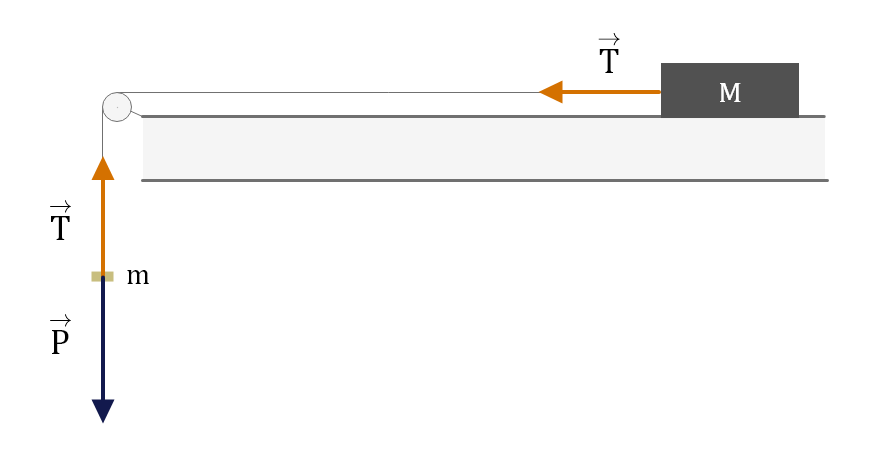
\includegraphics[scale=0.3]{force-diagram.png}
\centering
\caption{Diagramma delle forze}
\label{fig:forze}
\end{figure}

Il carrello si muove di moto rettilineo uniformemente accelerato e non risente delle forze di attrito.
Considerando $s_0=0$ e $t_0=0$ abbiamo:

\begin{equation}
    s=\frac{1}{2}at^2
\end{equation}

Da cui si ottiene $a=\frac{2s}{t^2}$.



Considerando le forze applicate al sistema negli assi x e y otterremo:

\begin{equation}
    \begin{cases}
    &T=Ma \quad \text{nell'asse x} \\
    &mg-T=ma \quad \text{nell'asse y}
    \end{cases}
\label{forze}
\end{equation}

In cui:
\begin{itemize}
    \item{$T$ è la tensione applicata sul filo, che in questo caso è anche la forza motrice del carrello sul piano}
    \item{$M$ indica la massa del carrello}
    \item{$a$ è l'accelerazione del carrello (e quindi anche delle massa in caduta)}
    \item{$m$ rappresenta la massa attaccata al filo, libera di muoversi verticalmente}
\end{itemize}
La prima equazione del sistema (\ref{forze}) esprime la seconda legge della dinamica sull'asse x in cui è assente la forza di attrito radente, in quanto annullata della spinta dell'aria sul carrello.
La seconda equazione del sistema (\ref{forze}) esprime, invece, la seconda legge della dinamica sull'asse y. In quest'equazione, oltre la tensione, compare la forza peso della massa applicata che ovviamente cadrà con accelerazione pari a quella del carrello.
Risolvendo il sistema si ottiene:

\begin{equation}
   M=\frac{m(g-a)}{a}=m \left( \frac{g}{a}-1\right).
\end{equation}

\section{Apparato sperimentale}
\subsection{Descrizione apparato}
Il macchinario è costituito da un carrello di massa M, su cui è agganciata un'estremità di un filo, che si solleva dalla guida tramite la pressione esercitata dall'aria grazie ad una pompa. Tra la guida e il carrello non è presente nessuna forza d'attrito. La rotaia è dotata di un’elettrocalamita di sgancio del carrello comandata da un pulsante che tiene il carrello fermo. La seconda estremità del filo è agganciata ad un gancio di massa $m_0$ al quale vengono applicate diverse masse ($m_1$, $m_2$, $m_3$, $m_4$). Al di sopra della guida sono posizionate 2 fotocellule disposte ad una distanza $s=s_1-s_2=0.670 \pm 0.002$ m, collegate ad un timer digitale con una sensibilità di 0.001 s.

\begin{figure}[H]
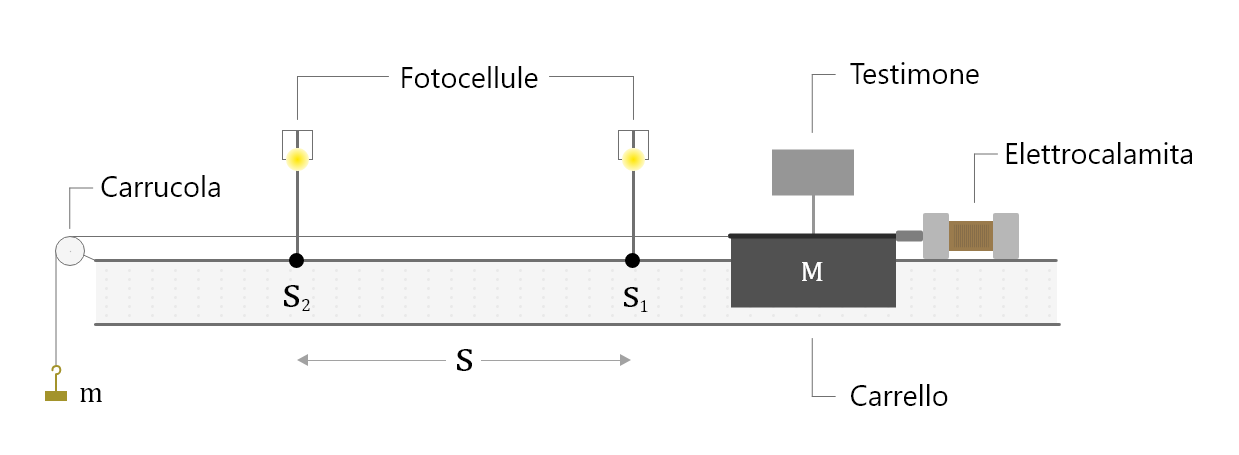
\includegraphics[scale=0.3]{experimental-setup.png}
\centering
\caption{Apparato sperimentale}
\label{fig:appspe}
\end{figure}

\subsection{Procedura di misura}
Per l'esperimento sono state utilizzate 5 masse diverse nelle seguenti configurazioni: $m_0$; $m_0+m_1$; $m_0+m_2$; $m_0+m_3$; $m_0+m_4$. Per ogni configurazione sono state effettuate 20 misure dell'intervallo di tempo $t$ impiegato per percorrere lo spazio $s$.

\begin{longtable}[]{@{}lllll@{}}
\toprule
Corpo & Massa (g) \tabularnewline
\midrule
\endhead
m0 & 9.85 $\pm$ 0.01 \tabularnewline
m1 & 10.23 $\pm$ 0.01 \tabularnewline
m2 & 20.10 $\pm$ 0.01 \tabularnewline
m3 & 30.33 $\pm$ 0.01 \tabularnewline
m4 & 40.21 $\pm$ 0.01 \tabularnewline
M & 296.5 $\pm$ 0.1 \tabularnewline
\bottomrule
\label{masses}
\end{longtable}

\subsection{Strumenti di misura}

\begin{longtable}[]{@{}lllll@{}}
\toprule
tool & uncertainty & uom \tabularnewline
\midrule
\endhead
Bilancia & 0.01 & g \tabularnewline
Metro & 0.001 & m \tabularnewline
Cronometro & 0.001 & s \tabularnewline
\bottomrule
\label{tools}
\end{longtable}

\section{Analisi dei dati e propagazione degli errori}
Dalla seconda legge della dinamica e secondo il diagramma delle forze illustrato in Figura \ref{fig:forze}
\begin{equation}
    \begin{cases}
    T=Ma \\
    mg-T=ma
    \end{cases}
    \Longrightarrow \; \; M=m \left( \frac{g}{a} -1 \right)
\end{equation}
Si procede alla propagazione degli errori

\begin{equation}
    \delta M = \left| \frac{\partial M}{\partial m_a} \right| \delta m_a + \left| \frac{\partial M}{\partial g} \right| \delta g + \left| \frac{\partial M}{\partial a} \right| \delta a
\end{equation}
Avendo $\delta m_a=2\delta m$ e $\delta a=\frac{2}{<t>^2}\left(\delta s + \frac{2}{<t>}\delta t \right)$ otteniamo:

\begin{equation}
    \delta M = \left( \frac{g}{a} -1 \right)2 \delta m + \frac{m}{a} \delta g + \frac{mg}{a^2}  \left [ \frac{2}{\langle t \rangle^2} \left( \delta s + \frac{2s}{\langle t \rangle}\delta t \right)\right]
\end{equation}

\section{Risultati e conclusioni}
 Come si può notare dalla figura 3 la dipendenza lineare tra forza e accelerazione è stata verificata, tuttavia il valore della massa del carrello non corrisponde esattamente a quello reale, infatti, \\dalla (4) si ottiene $M=m\left(\frac{g}{a}-1 \right) = 264 \pm 5 \; g $ \\mentre dalle misure effettuate con la bilancia, la massa del carrello, risulta essere $(296.5 \pm 0.1)g$
 
\begin{longtable}[]{@{}lllll@{}}
\toprule
configuration & acceleration ($m/s^2$) & relative error \tabularnewline
\midrule
\endhead
$m_0$ & 0.339 $\pm$ 0.002 & 0.59 \% \tabularnewline
$m_0+m_1$ & 0.688 $\pm$ 0.006 & 0.87 \% \tabularnewline
$m_0+m_2$ & 1.002 $\pm$ 0.008 & 0.80 \% \tabularnewline
$m_0+m_3$ & 1.320 $\pm$ 0.007 & 0.53 \% \tabularnewline
$m_0+m_4$ & 1.600 $\pm$ 0.009 & 0.56 \% \tabularnewline
\bottomrule
\label{output1}
\end{longtable}

\begin{longtable}[]{@{}lllll@{}}
\toprule
configuration & force (N) & relative error \tabularnewline
\midrule
\endhead
$m_0$ & 0.093 $\pm$ 0.001 & 1.08 \% \tabularnewline
$m_0+m_1$ & 0.183 $\pm$ 0.002 & 1.09 \% \tabularnewline
$m_0+m_2$ & 0.263 $\pm$ 0.003 & 1.14 \% \tabularnewline
$m_0+m_3$ & 0.341 $\pm$ 0.004 & 1.17 \% \tabularnewline
$m_0+m_4$ & 0.410 $\pm$ 0.006 & 1.46 \% \tabularnewline
\bottomrule
\label{output2}
\end{longtable}

\begin{longtable}[]{@{}lllll@{}}
\toprule
configuration & mass (g) & relative error \tabularnewline
\midrule
\endhead
$m_0$ & 275 $\pm$ 5 & 1.82 \% \tabularnewline
$m_0+m_1$ & 266 $\pm$ 6 & 2.26 \% \tabularnewline
$m_0+m_2$ & 263 $\pm$ 6 & 2.28 \% \tabularnewline
$m_0+m_3$ & 258 $\pm$ 5 & 1.94 \% \tabularnewline
$m_0+m_4$ & 256 $\pm$ 5 & 1.95 \% \tabularnewline
\bottomrule
\label{output3}
\end{longtable}

\begin{figure}[H]
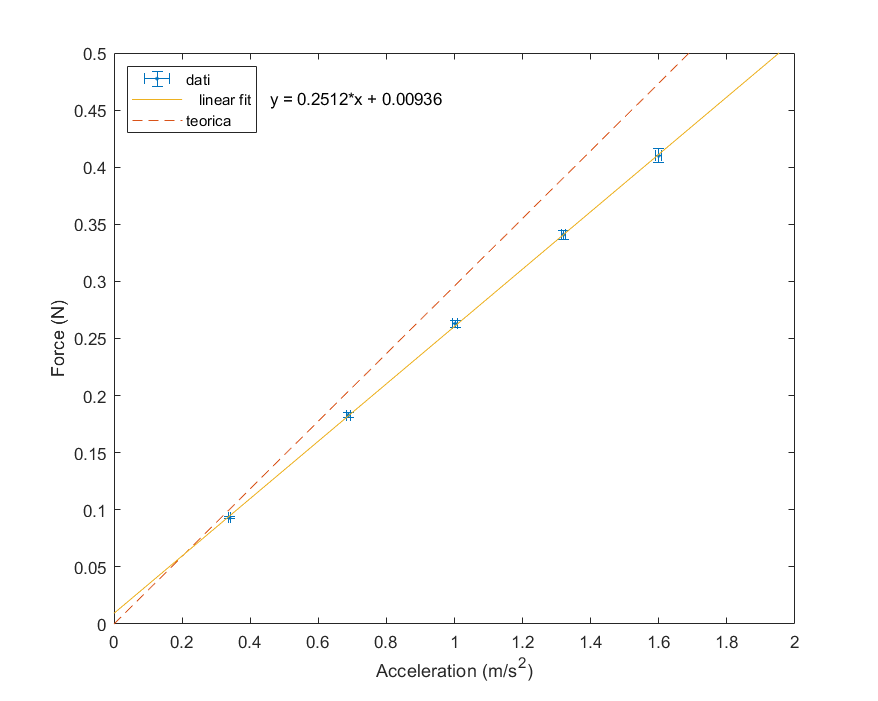
\includegraphics[scale=0.5]{plot-4.png}
\centering
\caption{Forza-accelerazione, correlazione lineare e retta teorica}
\label{plot:lincor}
\end{figure}

\section{Additional notes}

\subsection{Data Availability}
The data that support the findings of this study are openly available in \href{https://github.com/dennisangemi/lab1-dfa/tree/main/exp-3/data}{dennisangemi/lab1-dfa GitHub Repository} at \href{https://github.com/dennisangemi/lab1-dfa/tree/main/exp-3/data}{https://github.com/dennisangemi/lab1-dfa/tree/main/exp-3/data} under \href{https://creativecommons.org/licenses/by/4.0/}{CC-BY 4.0 license}.

\subsection{Code Availability}
The MATLAB code written to get the findings of this study is openly available in \href{https://github.com/dennisangemi/lab1-dfa/tree/main/exp-2/script}{dennisangemi/lab1-dfa GitHub Repository} at \href{https://github.com/dennisangemi/lab1-dfa/tree/main/exp-3/script}{https://github.com/dennisangemi/lab1-dfa/tree/main/exp-3/script}


\subsection{Software used}
\begin{itemize}
\item
  \textbf{MATLAB}: Data Analysis
\item
  \textbf{Google Spreadsheet}: Data entry
\item
  \textbf{Adobe Experience Design}: Images designing
\item
  \textbf{GitHub}: Resource sharing
\end{itemize}

\section{Bibliography}
\begin{itemize}
\item
  Taylor,~ J. (1999).~\emph{Introduzione all'analisi degli errori: Lo
  studio delle incertezze nelle misure fisiche.~}Zanichelli
\item
  Bevington P. (2002).~\emph{Data Reduction and Error Analysis for the
  Physical Sciences.~} McGraw-Hill Education ~
\item Malthe-Sørenssen, A. (2015). \emph{Elementary Mechanics Using Matlab: A Modern Course Combining Analytical and Numerical Techniques}. Springer
\end{itemize}

\section{Appendice A}
\subsection{Tabella \ref{expdata1}}

\begin{longtable}[]{@{}lllll@{}}
\toprule
dimension & value & uncertainty & uom \tabularnewline
\midrule
\endhead
s1 & 1.775 & 0.001 & MTR \tabularnewline
s2 & 1.105 & 0.001 & MTR \tabularnewline
s3 & 0.425 & 0.001 & MTR \tabularnewline
su & 0.539 & 0.001 & MTR \tabularnewline
m0 & 9.85 & 0.01 & GRM \tabularnewline
m1 & 10.23 & 0.01 & GRM \tabularnewline
m2 & 20.10 & 0.01 & GRM \tabularnewline
m3 & 30.33 & 0.01 & GRM \tabularnewline
m4 & 40.21 & 0.01 & GRM \tabularnewline
M & 296.5 & 0.1 & GRM \tabularnewline
\bottomrule
\label{expdata1}
\end{longtable}

\subsection{Tabella \ref{expdata2}}
\begin{longtable}[]{@{}lllll@{}}
\toprule
index & mass & t1 & uncertainty & uom  \tabularnewline
\midrule
\endhead
1 & $m_0$ & 1.983 & 0.001 & SEC \tabularnewline
2 & $m_0$ & 1.983 & 0.001 & SEC \tabularnewline
3 & $m_0$ & 1.981 & 0.001 & SEC \tabularnewline
4 & $m_0$ & 1.989 & 0.001 & SEC \tabularnewline
5 & $m_0$ & 1.990 & 0.001 & SEC \tabularnewline
6 & $m_0$ & 1.984 & 0.001 & SEC \tabularnewline
7 & $m_0$ & 1.988 & 0.001 & SEC \tabularnewline
8 & $m_0$ & 1.991 & 0.001 & SEC \tabularnewline
9 & $m_0$ & 1.984 & 0.001 & SEC \tabularnewline
10 & $m_0$ & 1.990 & 0.001 & SEC \tabularnewline
11 & $m_0$ & 1.990 & 0.001 & SEC \tabularnewline
12 & $m_0$ & 1.993 & 0.001 & SEC \tabularnewline
13 & $m_0$ & 1.987 & 0.001 & SEC \tabularnewline
14 & $m_0$ & 1.985 & 0.001 & SEC \tabularnewline
15 & $m_0$ & 1.994 & 0.001 & SEC \tabularnewline
16 & $m_0$ & 1.986 & 0.001 & SEC \tabularnewline
17 & $m_0$ & 1.982 & 0.001 & SEC \tabularnewline
18 & $m_0$ & 1.984 & 0.001 & SEC \tabularnewline
19 & $m_0$ & 1.998 & 0.001 & SEC \tabularnewline
20 & $m_0$ & 1.985 & 0.001 & SEC \tabularnewline
1 & $m_0$+$m_1$ & 1.402 & 0.001 & SEC \tabularnewline
2 & $m_0$+$m_1$ & 1.400 & 0.001 & SEC \tabularnewline
3 & $m_0$+$m_1$ & 1.400 & 0.001 & SEC \tabularnewline
4 & $m_0$+$m_1$ & 1.402 & 0.001 & SEC \tabularnewline
5 & $m_0$+$m_1$ & 1.404 & 0.001 & SEC \tabularnewline
6 & $m_0$+$m_1$ & 1.389 & 0.001 & SEC \tabularnewline
7 & $m_0$+$m_1$ & 1.393 & 0.001 & SEC \tabularnewline
8 & $m_0$+$m_1$ & 1.396 & 0.001 & SEC \tabularnewline
9 & $m_0$+$m_1$ & 1.390 & 0.001 & SEC \tabularnewline
10 & $m_0$+$m_1$ & 1.402 & 0.001 & SEC \tabularnewline
11 & $m_0$+$m_1$ & 1.389 & 0.001 & SEC \tabularnewline
12 & $m_0$+$m_1$ & 1.402 & 0.001 & SEC \tabularnewline
13 & $m_0$+$m_1$ & 1.390 & 0.001 & SEC \tabularnewline
14 & $m_0$+$m_1$ & 1.393 & 0.001 & SEC \tabularnewline
15 & $m_0$+$m_1$ & 1.393 & 0.001 & SEC \tabularnewline
16 & $m_0$+$m_1$ & 1.394 & 0.001 & SEC \tabularnewline
17 & $m_0$+$m_1$ & 1.394 & 0.001 & SEC \tabularnewline
18 & $m_0$+$m_1$ & 1.394 & 0.001 & SEC \tabularnewline
19 & $m_0$+$m_1$ & 1.392 & 0.001 & SEC \tabularnewline
20 & $m_0$+$m_1$ & 1.394 & 0.001 & SEC \tabularnewline
1 & $m_0$+$m_2$ & 1.151 & 0.001 & SEC \tabularnewline
2 & $m_0$+$m_2$ & 1.154 & 0.001 & SEC \tabularnewline
3 & $m_0$+$m_2$ & 1.159 & 0.001 & SEC \tabularnewline
4 & $m_0$+$m_2$ & 1.159 & 0.001 & SEC \tabularnewline
5 & $m_0$+$m_2$ & 1.159 & 0.001 & SEC \tabularnewline
6 & $m_0$+$m_2$ & 1.161 & 0.001 & SEC \tabularnewline
7 & $m_0$+$m_2$ & 1.154 & 0.001 & SEC \tabularnewline
8 & $m_0$+$m_2$ & 1.152 & 0.001 & SEC \tabularnewline
9 & $m_0$+$m_2$ & 1.154 & 0.001 & SEC \tabularnewline
10 & $m_0$+$m_2$ & 1.151 & 0.001 & SEC \tabularnewline
11 & $m_0$+$m_2$ & 1.152 & 0.001 & SEC \tabularnewline
12 & $m_0$+$m_2$ & 1.158 & 0.001 & SEC \tabularnewline
13 & $m_0$+$m_2$ & 1.158 & 0.001 & SEC \tabularnewline
14 & $m_0$+$m_2$ & 1.160 & 0.001 & SEC \tabularnewline
15 & $m_0$+$m_2$ & 1.161 & 0.001 & SEC \tabularnewline
16 & $m_0$+$m_2$ & 1.159 & 0.001 & SEC \tabularnewline
17 & $m_0$+$m_2$ & 1.159 & 0.001 & SEC \tabularnewline
18 & $m_0$+$m_2$ & 1.157 & 0.001 & SEC \tabularnewline
19 & $m_0$+$m_2$ & 1.154 & 0.001 & SEC \tabularnewline
20 & $m_0$+$m_2$ & 1.152 & 0.001 & SEC \tabularnewline
1 & $m_0$+$m_3$ & 1.012 & 0.001 & SEC \tabularnewline
2 & $m_0$+$m_3$ & 1.010 & 0.001 & SEC \tabularnewline
3 & $m_0$+$m_3$ & 1.010 & 0.001 & SEC \tabularnewline
4 & $m_0$+$m_3$ & 1.009 & 0.001 & SEC \tabularnewline
5 & $m_0$+$m_3$ & 1.008 & 0.001 & SEC \tabularnewline
6 & $m_0$+$m_3$ & 1.009 & 0.001 & SEC \tabularnewline
7 & $m_0$+$m_3$ & 1.010 & 0.001 & SEC \tabularnewline
8 & $m_0$+$m_3$ & 1.009 & 0.001 & SEC \tabularnewline
9 & $m_0$+$m_3$ & 1.009 & 0.001 & SEC \tabularnewline
10 & $m_0$+$m_3$ & 1.008 & 0.001 & SEC \tabularnewline
11 & $m_0$+$m_3$ & 1.006 & 0.001 & SEC \tabularnewline
12 & $m_0$+$m_3$ & 1.007 & 0.001 & SEC \tabularnewline
13 & $m_0$+$m_3$ & 1.007 & 0.001 & SEC \tabularnewline
14 & $m_0$+$m_3$ & 1.008 & 0.001 & SEC \tabularnewline
15 & $m_0$+$m_3$ & 1.006 & 0.001 & SEC \tabularnewline
16 & $m_0$+$m_3$ & 1.006 & 0.001 & SEC \tabularnewline
17 & $m_0$+$m_3$ & 1.005 & 0.001 & SEC \tabularnewline
18 & $m_0$+$m_3$ & 1.005 & 0.001 & SEC \tabularnewline
19 & $m_0$+$m_3$ & 1.004 & 0.001 & SEC \tabularnewline
20 & $m_0$+$m_3$ & 1.005 & 0.001 & SEC \tabularnewline
1 & $m_0$+$m_4$ & 0.913 & 0.001 & SEC \tabularnewline
2 & $m_0$+$m_4$ & 0.913 & 0.001 & SEC \tabularnewline
3 & $m_0$+$m_4$ & 0.914 & 0.001 & SEC \tabularnewline
4 & $m_0$+$m_4$ & 0.913 & 0.001 & SEC \tabularnewline
5 & $m_0$+$m_4$ & 0.914 & 0.001 & SEC \tabularnewline
6 & $m_0$+$m_4$ & 0.915 & 0.001 & SEC \tabularnewline
7 & $m_0$+$m_4$ & 0.912 & 0.001 & SEC \tabularnewline
8 & $m_0$+$m_4$ & 0.914 & 0.001 & SEC \tabularnewline
9 & $m_0$+$m_4$ & 0.914 & 0.001 & SEC \tabularnewline
10 & $m_0$+$m_4$ & 0.916 & 0.001 & SEC \tabularnewline
11 & $m_0$+$m_4$ & 0.918 & 0.001 & SEC \tabularnewline
12 & $m_0$+$m_4$ & 0.918 & 0.001 & SEC \tabularnewline
13 & $m_0$+$m_4$ & 0.915 & 0.001 & SEC \tabularnewline
14 & $m_0$+$m_4$ & 0.918 & 0.001 & SEC \tabularnewline
15 & $m_0$+$m_4$ & 0.918 & 0.001 & SEC \tabularnewline
16 & $m_0$+$m_4$ & 0.915 & 0.001 & SEC \tabularnewline
17 & $m_0$+$m_4$ & 0.915 & 0.001 & SEC \tabularnewline
18 & $m_0$+$m_4$ & 0.915 & 0.001 & SEC \tabularnewline
19 & $m_0$+$m_4$ & 0.915 & 0.001 & SEC \tabularnewline
20 & $m_0$+$m_4$ & 0.916 & 0.001 & SEC \tabularnewline
\bottomrule
\label{expdata2}
\end{longtable}

\end{document}
